\documentclass{beamer}
\usepackage{amsmath}

\title{Solution to Differential Equation}
\subtitle{EE24BTECH11012 - Bhavanisankar G S}
\date{\today}

\begin{document}

\frame{\titlepage}

\begin{frame}
\frametitle{Problem Statement}
For the differential equation \( x(x^2 - 1) \frac{dy}{dx} = 1 \), find the particular solution given \( y(2) = 0 \).
\end{frame}

\begin{frame}
\frametitle{Theoretical Solution - 1}
\[
\frac{dy}{dx} = \frac{1}{x(x^2 - 1)}
\]
Using partial fractions:
\[
\frac{dy}{dx} = \frac{1}{2} \left(\frac{1}{x-1} + \frac{1}{x+1}\right) - \frac{1}{x}
\]
\end{frame}

\begin{frame}
\frametitle{Theoretical Solution - 2}
Integrating both sides:
\[
y = \frac{1}{2} \log |x - 1| + \frac{1}{2} \log |x + 1| - \log |x| + \log c
\]
\end{frame}

\begin{frame}
\frametitle{Applying Initial Condition}
Substituting \( y(2) = 0 \):
\[
0 = \log \left( c \sqrt{\frac{3}{4}} \right)
\]
Solving for \( c \):
\[
c = 2\sqrt{3}
\]
\end{frame}

\begin{frame}
\frametitle{Particular Solution}
The particular solution becomes:
\[
y = \log \left( 2\sqrt{\frac{x^2 - 1}{3x}} \right)
\]
\end{frame}

\begin{frame}
\frametitle{Simulation - Trapezoid Rule}
For a general interval, say \(\sbrak{a,b}\), split up the intervals into \(n\) parts such that
\begin{align}
	h &= \frac{b-a}{n}
\end{align}
Consider the points:
\begin{align}
	x_{0} &= a \\
	x_{n} &= b \\
	x_{i+1} &= x_{i} + h
\end{align}
\end{frame}

\begin{frame}
\frametitle{Difference Equation}
Deriving the difference equation:
\begin{align}
	f(x) &= \frac{1}{x \left( {x^2 - 1}} \right) \\
	A &\approx \frac{h}{2} \left( {(f(x_{0}) + f(x_{1})) + (f(x_{1}) + f(x_{2})) + \dots + (f(x_{n-1}) + f(x_{n}))} \right) \\
	A &\approx \frac{h}{2} \left( {f(x_{0}) + 2 \sum_{i=1}^{n-1} f(x_{i}) + f(x_{n}) } \right)
\end{align}
On further simplifying, we have
\begin{align}
	y_{n+1} - y_{n} &= \left( {x_{n+1} - x_{n}}  \right) \left( {\frac{f(x_{n})}{2} + \frac{f(x_{n+1}) }{2}} \right) \\
	y_{n+1} &= y_{n} + \left( {x_{n+1} - x_{n}}  \right)\left( {\frac{f(x_{n})}{2} + \frac{f(x_{n+1})}{2} \right) } \\
	y_{n+1} &= y_{n} + \frac{\left( {x_{n+1} - x_{n}}}{2} \right) \left({\frac{1}{x_{n}(x_{n}^2 - 1)} + \frac{1}{x_{n+1}(x_{n+1}^2 - 1) } \right)}
\end{align}
which is the required difference equation.
\end{frame}

\begin{frame}
\frametitle{Laplace Transform Approach}
\begin{align}
	g(t) &= \frac{1}{t(t^2 - 1)} \\
	\frac{dy}{dt} &= g(t) \\
	s Y(s) &= X(s) \\
	H(s) &= \frac{Y(s)}{X(s)} \\
	H(s) &= \frac{1}{s}
\end{align}
\end{frame}

\begin{frame}
\frametitle{Bilinear Transform}
\begin{align}
	s &= \frac{2}{h} \left( {\frac{1 - z^{-1}}{1 + z^{-1}}} \right)  \\
	H(z) &= \frac{h}{2} \left( {\frac{1 + z^{-1}}{1 - z^{-1}}} \right) \\
	Y(z) &= \frac{h}{2} \left( {\frac{1 + z^{-1}}{1 - z^{-1}}} \right) X(z) , |z| > 1\\
	\left( {1 - z^{-1}} \right) Y(z) &= \frac{h}{2} \left( \brak{1 + z^{-1}} \right) X(z) 
\end{align}
Taking inverse \(z\)-transform on both sides, we have
\begin{align}
	y_{n} - y_{n-1} &= \frac{h}{2} \left( {g(x_{n}) + g(x_{n-1})} \right) \\
	y_{n} &= y_{n-1} + \frac{h}{2} \left( {g(x_{n}) + g(x_{n-1})} \right)
\end{align}
\end{frame}

\begin{frame}
\frametitle{Runge-Kutta Method}
\begin{align}
	y(x + h) &= y(x) + y^{\prime}(x,y) h \\
	y^{\prime} (x,y) &= \frac{1}{x \left( {x^2 - 1} \right)} \\
	y(x_0 + h) &= y(x_0) + \frac{1}{6} \left( {k_1 + 2k_2 + 2k_3 + k_4} \right)
\end{align}
where,
\begin{align}
	k_1 &= h y^{\prime} ({x_0, y_0}) \\
	k_2 &= h y^{\prime} ({x_0 + \frac{h}{2}, y_0 + \frac{k_1}{2}}) \\
	k_3 &= h y^{\prime} \left( {x_0 + \frac{h}{2}, y_0 + \frac{k_2}{2}} \right)\\
	k_4 &= h y^{\prime} \left( {x_0 + h, y_0 + k_3} \right)
\end{align}
\end{frame}

\begin{frame}
\frametitle{Graphical Representation}
\begin{figure}[h]
	\centering
	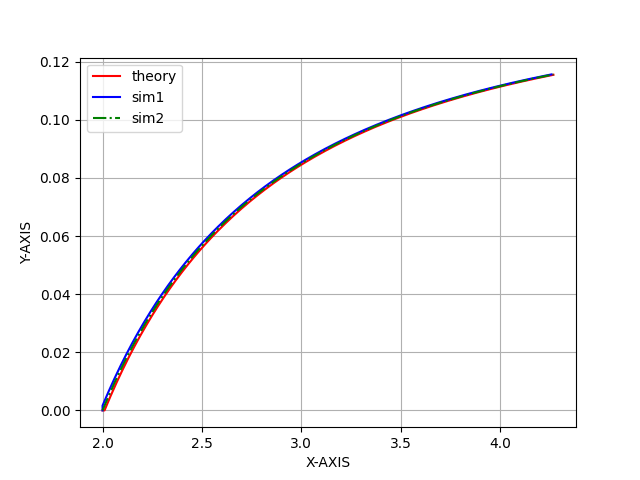
\includegraphics[width=\columnwidth]{fig.png}
	\caption{Plot of the given question.}
	\label{fig:Plot1}
\end{figure}
\end{frame}

\end{document}

